\iffalse
\chapter{2023}
\author{AI24BTECH11020}
\section{ae}
\fi

%\begin{enumerate}[start=40]
	\item Consider a general aviation airplane with weight $10 kN$ and a wing platform area of $15 m^2$. The drag coefficient of the airplane is given as $C_D=C_{D_0}+KC_L^2$ with $C_{D_0}=0.025$ and $K=0.05$. For level flight at an altitude where the destiny is $0.60 kg/m^3$ and thrust $1 kN$, the maximum cruise speed is (rounded off to the nearest integer)
		\begin{enumerate}
			\item $87 m/s$
			\item $30 m/s$
			\item $36 m/s$
			\item $101 m/s$
		\end{enumerate}


	\item A scramjet engine features an intake ,isolator, combustor and a nozzle, as shown in the schematic. Station $3$ indicates the combustor entry point. Assume stagnation enthalpy to be constant between Stations $1$ and $3$, and air to be a calorically perfect gas with specific heat ratio $\gamma$. Select the correct expression for Mach number $M_3$ at the inlet to the combustor from the options given.\\
		\begin{center}		
\begin{tikzpicture}[font=\large, scale=0.5]
    \draw (5,14.75) -- (22.25,14.75);
    \draw (9.5,10.25) -- (18.25,10.25);
    \draw (9.5,9.25) -- (17.75,9.25);
    \draw (2.5,14.75) -- (5,14.75);
    \draw (2.5,14.75) -- (6,13.5);
    \draw (6,13.5) -- (9.5,10.25);
    \draw (22.25,14.75) -- (20.25,13.75);
    \draw (20.25,13.75) -- (18.25,10.25);
    \draw[dashed] (18.5,14.75) -- (18.25,10.25);
    \draw[dashed] (14.75,14.75) -- (14.75,10.25);
    \draw[dashed] (9.5,14.75) -- (9.5,10.5);
    \draw[dashed] (2.5,16) -- (2.5,14.75);
    \draw (9.25,9.5) -- (9.5,9.25);
    \draw (9.25,9.75) -- (6,13.5);
    \draw (9.25,9.5) -- (9.25,9.75);
    \draw (9.25,9.75) -- (9.5,10.25);
    \draw (9.5,9.25) -- (9.5,10.25);
    \draw (9.5,10.25) -- (11.5,9.25);
    \draw (11.5,9.25) -- (12.75,10.25);
    \draw (12.75,10.25) -- (14,9.25);
    \draw (14,9.25) -- (15,10.25);
    \draw (2.5,14.75) -- (9,10);
    \node at (3,15.75) {1};
    \node at (9.5,15.25) {2};
    \node at (14.75,15.25) {3};
    \node at (18.5,15.25) {4};
    \draw[dashed] (22,16.5) -- (22,14.75);
    \node at (22.5,15.25) {5};
    \node at (4,11.5) {Free stream};
    \fill[black] (15,10)--(15.4,10.1)--(15.4,9.9)--(15,10);
    \fill[black] (15,9.5)--(15.4,9.6)--(15.4,9.4)--(15,9.5);
    \shade[left color=yellow, right color=orange] (15.8,10) rectangle (18,9.4); 
    \draw[->, >=Stealth] (2,11) -- (6.5,11);
    \node at (4.75,10.25) {$M_\infty, T_\infty, P_\infty$};
\end{tikzpicture}
		\end{center}
		\begin{enumerate}
			\item $M_3=M_{\infty}\sqrt{\brak{\frac{2}{\gamma-1}}\brak{\frac{T_{\infty}}{T_3}-1}}$
			\item $M_3=\sqrt{\brak{\frac{2}{\gamma-1}}\cbrak{\frac{T_{\infty}}{T_3}\sbrak{1+\brak{\frac{\gamma-1}{2}}M_{\infty}^2}-1}}$
			\item $M_3=M_{\infty}\sqrt{\frac{T_{\infty}}{T_3}}$
			\item $M_3=\sqrt{\brak{\frac{\gamma+1}{2}}\brak{\frac{T_{\infty}}{T_3}-1}M_{\infty}^2-1}$
		\end{enumerate}


	\item Consider the equation $\frac{dy}{dx}+\alpha y=\sin \omega x$, where $\alpha$ and $\omega$ are constants. Given $y=1$ at $x=0$, select all correct statements(s) from the following as $x \to \infty$.
		\begin{enumerate}
	\item $y\to 0$ if $\alpha\neq0$
	\item $y\to 1$ if $\alpha =0$
	\item $y\to A exp\brak{\abs{\alpha}x}$ if $\alpha<0;A$ is a constant
	\item $y\to B \sin\brak{\omega x+C}$ if $\alpha>0;B$ and $C$ are constants
		\end{enumerate}


	\item Given the vectors \\ $\vec{A}=9\hat{i}-5\hat{j}+2\hat{k}\\ \vec{B}=11\hat{i}+4\hat{j}+\hat{k}\\ \vec{C}=-7\hat{i}+14\hat{j}-3\hat{k}$\\ which of the following statement(s) is/are TRUE?
		\begin{enumerate}
		\item Vectors $A,B$ and $C$ are coplanar
		\item The scalar triple product of the vectors $A,B$ and $C$ is zero
		\item $A$ and $B$ are perpendicular
		\item $C$ is parallel to $A \times B$
		\end{enumerate}

		
	\item Consider a one-dimensional inviscid supersonic flow in a diverging duct with heat addition($Q_m$) as shown. Which of the following statement(s) is/are always TRUE?\\
		\begin{center}
    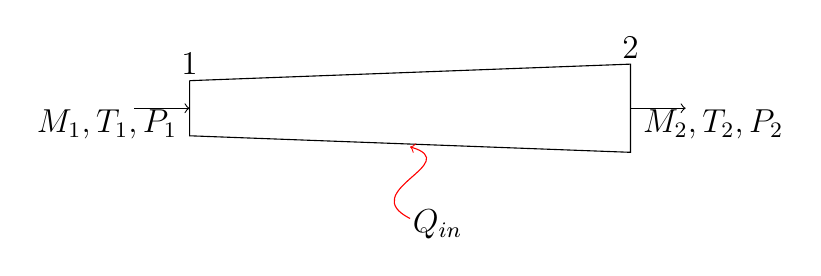
\begin{tikzpicture}[font=\large, scale=0.7]
        \draw (0,0.5)--(8,0.8)--(8,-0.8)--(0,-0.5)--(0,0.5);
    \draw[->] (8,0)--(9,0);
    \draw[->] (-1,0)--(0,0);
    \node at (0,0.8){$1$};
    \node at (8,1.1) {$2$};
    \node at (9.5,-0.3) {$M_2,T_2,P_2$};
    \node at (-1.5,-0.3) {$M_1,T_1,P_1$};
    \draw[color=red][->] (4,-2) .. controls (3,-1.5) and (5,-1) .. (4,-0.7);
    \node at (4.5,-2.1){$Q_{in}$};
    \end{tikzpicture}
\end{center}
		\begin{enumerate}
			\item Mach number, $M_2>M_1$
			\item Stagnation pressure, $P_1\degree>P_2\degree$
			\item Static pressure, $P_2>P_1$
			\item Stagnation temperature, $T_1\degree<T_2\degree$
		\end{enumerate}

	\item Consider the International Standard Atmosphere (ISA) with $h$ being the geopotential altitude (in $km$) and $\frac{dT}{dh}$ being the temperature gradient (in $K/m$). Which of the following combination(s) of, $\brak{h,\frac{dT}{dh}}$ is/are as per ISA?
		\begin{enumerate}
			\item $\brak{7,-6.5\times10^{-3}}$
			\item $\brak{9,4\times10^{-3}}$
			\item $\brak{15,0}$
			\item $\brak{35,3\times10^{-3}}$
		\end{enumerate}

		
	\item For an airfoil, which of the relations given about the critical Mach number $M_{cr}$ and drag divergence Mach number $M_{dd}$ is/are correct?
		\begin{enumerate}
			\item $M_{cr}<M_{dd}$
			\item $M_{cr}<1.0$
			\item $M_{dd}<1.0$
			\item $M_{cr}>1.0$
		\end{enumerate}

	\item Which of the following statement(s) about the elastic flexural buckling load of columns is/are correct?
		\begin{enumerate}
			\item The buckling load increases with increase in flexural rigidity of the column.
			\item The buckling load increases with increase in the length of the column.
			\item The boundary conditions of the column affect the buckling load
			\item The buckling load is NOT directly dependent on the density of the material used for the column.
		\end{enumerate}


	\item The thickness of a uniform hollow circular shaft is equal to the difference between the outer radius and the inner radius. The ratio of the inner diameter to outer diameter of the shaft is $0.5$. For the shaft reacting to an applied torque, the ratio of
the maximum shear stress $\tau$ to the maximum shear stress $\tau_{thin-wall}$ obtained using the thin-wall approximation is \underline{\hspace{2cm}} . (round off to one decimal place)
        \item A rigid bar $AB$ is subjected to a uniformly distributed load of $100 N/m$ as shown in the figure. The bar is supported by rod $CD$, with $A, C,$ and $D$ as pin joints. The rod $CD$ has axial stiffness of $40 N/mm$. The vertical deflection at point $D$ is \underline{\hspace{2cm}} $mm$. (round off to nearest integer)\\
		\begin{center}
			\begin{tikzpicture}[font=\Large, scale=0.8]
\draw (8.75,15.75) -- (15,15.75);
\draw (8.75,15.75) -- (8.75,14.75);
\draw (8.75,14.75) -- (16.75,14.75);
\draw (16.75,14.75) -- (16.75,15.75);
\draw (14.75,15.75) -- (16.75,15.75);
\foreach \x in {9, 9.75, 10.5, 11.25, 12, 12.75, 13.5, 14.25, 15, 16, 16.75} {
    \draw[->, >=Stealth] (\x,15.75) -- (\x,16.75);
}
\draw (7.5,16.75) rectangle (8.75,9.25);
\draw (8.75,12.25) -- (12.75,15.25);
\draw (6.5,15.5) -- (7.5,15.5);
\draw (7,15.5) -- (7,14.25);
\draw (7,13.75) -- (7,12.25);
\draw (6.25,12.25) -- (7.5,12.25);
\draw (6.5,15.5) -- (6.25,15.5);
\node[font=\large] at (7,13.75) {1m};
\draw (8.75,14.5) -- (8.75,13.75);
\draw (8.75,14) -- (10,14);
\draw (12.75,14.25) -- (12.75,13.5);
\draw (16.75,14.25) -- (16.75,13.5);
\draw (11.25,14) -- (14.25,14);
\draw (12.75,14.25) -- (12.75,14.5);
\draw (16.75,14) -- (16.75,14.5);
\node[font=\large] at (10.75,14) {1m};
\node[font=\large] at (14.75,14) {1m};
\draw (15.25,14) -- (16.75,14);
\node[font=\large] at (9.5,15.25) {$A$};
\node[font=\large] at (17.25,15.25) {$B$};
\node at (18,16.5){$100 N/m$};
\node[font=\large] at (9,12){$C$};
\node[font=\large] at (13,15.25){$D$};
\end{tikzpicture}
		\end{center}

	\item A cantilever beam of length $2a$ is loaded at the tip with force $F$ as shown in the figure. The beam is supported in the middle by a roller with a pin. The magnitude of moment reaction at the built-in end of the beam is $\alpha Fa$, where $\alpha$ is \underline{\hspace{2cm}}. (round off to one decimal place)\\
		\begin{figure}[!ht]
\centering
\resizebox{0.6\textwidth}{!}{%
\begin{circuitikz}
\tikzstyle{every node}=[font=\LARGE]
\draw [line width=0.6pt, short] (5.75,11) -- (19.5,11);
\draw [line width=0.5pt, short] (5.75,10.25) -- (19.5,10.25);
\draw [line width=0.3pt, short] (5.75,13) -- (5.75,10.25);
\draw [line width=0.3pt, short] (12.75,13) -- (12.75,11.25);
\draw [line width=0.9pt, short] (4.75,12) -- (4.5,11.75);
\draw [line width=0.9pt, short] (5,12) -- (4.5,11.5);
\draw [line width=0.9pt, short] (5.25,12) -- (4.5,11.25);
\draw [line width=0.9pt, short] (5.5,12) -- (4.5,11);
\draw [line width=0.9pt, short] (5.75,12) -- (4.5,10.75);
\draw [line width=0.9pt, short] (5.75,11.75) -- (4.5,10.5);
\draw [line width=0.9pt, short] (5.75,11.5) -- (4.5,10.25);
\draw [line width=0.9pt, short] (5.75,11) -- (4.75,10);
\draw [line width=0.9pt, short] (5.75,11.25) -- (4.5,10);
\draw [line width=0.9pt, short] (5.75,10.75) -- (5,10);
\draw [line width=0.9pt, short] (5.75,10.5) -- (5.25,10);
\draw [line width=0.9pt, short] (5.75,10.25) -- (5.5,10);

%triangle
\draw [line width=0.9pt, short] (12.75,10.75) -- (12,9.5);
\draw [line width=0.9pt, short] (12.75,10.75) -- (13.5,9.5);
\draw [line width=0.9pt, short] (12,9.5) -- (13.5,9.5);

\fill (12.75,10.75) circle (3pt); 
\fill (12.2,9.36) circle (4.8pt);     
\fill (13.3,9.36) circle (4.8pt);   

\draw [line width=2pt, ->, >=Stealth] (19.25,14.75) -- (19.25,11.25);
\node [font=\LARGE] at (20.25,14) {F};
\draw [line width=1pt, <->, >=Stealth] (5.75,12) -- (12.75,12)node[pos=0.55, fill=white]{a};
\draw [line width=1pt, <->, >=Stealth] (12.75,12) -- (19.25,12)node[pos=0.55, fill=white]{a};
\draw [line width=1pt, short] (19.5,11) -- (19.5,10.25);
\draw [line width=1pt, short] (11.75,9.25) -- (11.5,9);
\draw [line width=1pt, short] (12,9.25) -- (11.75,9);
\draw [line width=1pt, short] (12.25,9.25) -- (12,9);
\draw [line width=1pt, short] (12.5,9.25) -- (12.25,9);
\draw [line width=1pt, short] (12.75,9.25) -- (12.5,9);
\draw [line width=1pt, short] (13,9.25) -- (12.75,9);
\draw [line width=1pt, short] (13.25,9.25) -- (13,9);
\draw [line width=1pt, short] (13.5,9.25) -- (13.25,9);
\draw [line width=1pt, short] (13.75,9.25) -- (13.5,9);
\end{circuitikz}
}%
\end{figure}

	\item A single degree-of-freedom spring-mass-damper system has viscous damping ratio of $0.1$. The mass is given an initial displacement of $10 cm$ without imparting any velocity. After exactly two complete cycles of oscillation (i.e., after time $2T_d$ , where $T_d$ is the period of the damped vibration), the amplitude of the displacement is\underline{\hspace{2cm}} $cm$. (round off to two decimal place)
	
	\item The shear flow distribution in a single cell, thin-walled beam under the action of an arbitrary shear load $s_y$ applied at the shear centre $S$ is shown in the figure. The cell has horizontal symmetry with booms marked by $1$ to $4$ that carry direct stresses. The shear modulus $G$ is the same for all the walls, and the area of the cell is $135000 mm^2$. With respect to the point $O$ marked in the figure, the distance to the shear centre $S$ is \underline{\hspace{2cm}} $mm$. (round off to the nearest integer)\\
		\begin{center}
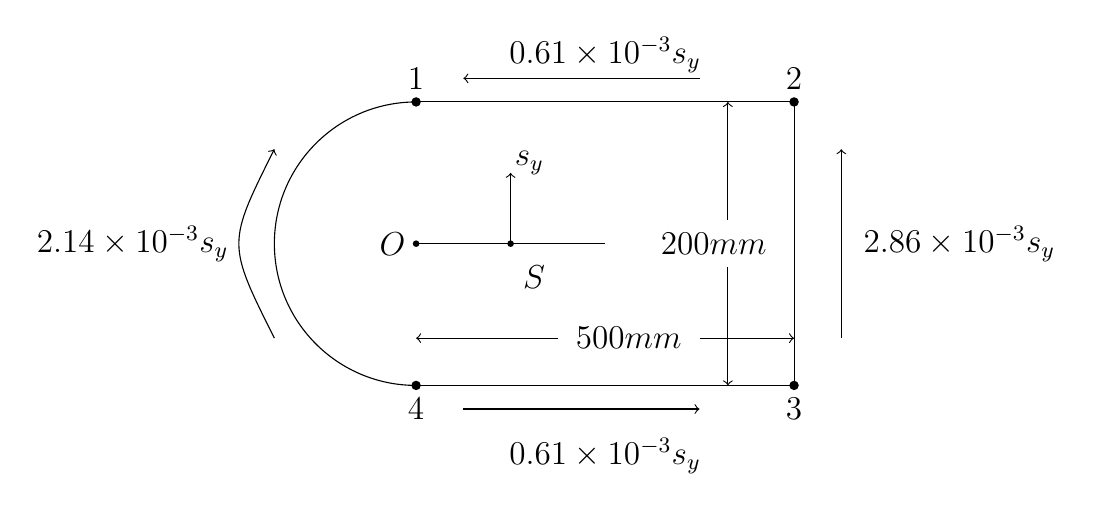
\begin{tikzpicture}[font=\large, scale=0.6]
    \draw (0,0)--(8,0)--(8,-6)--(0,-6);
    \draw (0,0) arc[start angle=90, end angle=270,radius=3cm];
    \draw[->] (-3,-5)..controls (-4,-3)..(-3,-1);
    \node at (-6,-3){$2.14\times 10^{-3}s_y$};
    \fill[black](0,-3) circle (0.7mm);
    \node at (-0.5,-3){$O$}; 
    \node at (0,0.5){$1$};\fill[black](0,0) circle (1mm);
    \node at (0,-6.5){$4$};\fill[black](0,-6) circle (1mm);
    \node at (8,0.5){$2$};\fill[black](8,0) circle (1mm);
    \node at (8,-6.5){$3$};\fill[black](8,-6) circle (1mm);
    \node at (2.5,-3.7){$S$};\fill[black](2,-3) circle (0.7mm);
    \draw (0,-3)--(4,-3);
    \draw[<-] (1,0.5)--(6,0.5);\node at (4,1){$0.61\times 10^{-3}s_y$};
    \draw[->] (1,-6.5)--(6,-6.5);\node at (4,-7.5){$0.61\times 10^{-3}s_y$};
    \draw[<-] (9,-1)--(9,-5);\node at (11.5,-3){$2.86\times10^{-3}s_y$};
    \draw[<-] (0,-5)-- (3,-5);\node at (4.5,-5){$500 mm$};
    \draw[->] (6,-5)--(8,-5);
    \draw[<-] (6.6,0)-- (6.6,-2.5);\node at (6.3,-3){$200 mm$};
    \draw[->] (6.6,-3.5)--(6.6,-6);
    \draw[->](2,-3)--(2,-1.5);
    \node at (2.4,-1.3) {$s_y$}; 
\end{tikzpicture}
\end{center}


%\end{enumerate}

